% Based on http://www-i6.informatik.rwth-aachen.de/~dreuw/latexbeamerposter.php
\documentclass[final]{beamer} % beamer 3.10: do NOT use option hyperref={pdfpagelabels=false} !
  %\documentclass[final,hyperref={pdfpagelabels=false}]{beamer} % beamer 3.07: get rid of beamer warnings
  \mode<presentation> {  %% check http://www-i6.informatik.rwth-aachen.de/~dreuw/latexbeamerposter.php for examples
    \usetheme{knauss-v01}    %% you should define your own theme e.g. for big headlines using your own logos 
  }
  \usepackage[english]{babel}
  %\usepackage[latin1]{inputenc}
  \usepackage{amsmath,amsthm, amssymb, latexsym}
  %\usepackage{times}\usefonttheme{professionalfonts}  % times is obsolete
  \usefonttheme[onlymath]{serif}
  \boldmath
  \usepackage[english]{babel}
  \usepackage[utf8]{inputenc}
  \usepackage[orientation=portrait,size=a4,scale=0.5,debug]{beamerposter} 
  \usepackage{tabularx}
  \usepackage{booktabs}
  \usepackage{array}
  \usepackage{subfig}
  \newcolumntype{v}[1]{>{\raggedright \hspace {0pt}}p{#1}}
  \newcolumntype{V}[1]{>{\centering \hspace {0pt}}p{#1}}
  
  \newcommand{\marker}[1]{\textbf{\color{knaccentcolor1} #1}}
  
  % e.g. for DIN-A0 poster
  %\usepackage[orientation=portrait,size=a1,scale=1.4,grid,debug]{beamerposter}                  % e.g. for DIN-A1 poster, with optional grid and debug output
  %\usepackage[size=custom,width=200,height=120,scale=2,debug]{beamerposter}                     % e.g. for custom size poster
  %\usepackage[orientation=portrait,size=a0,scale=1.0,printer=rwth-glossy-uv.df]{beamerposter}   % e.g. for DIN-A0 poster with rwth-glossy-uv printer check
  % ...
  %
  \title[Requirements Patterns]{Patterns of Requirements related Communication}
  \author[Knauss]{Eric Knauss*}
  \institute[University of Victoria]{University of Victoria, Canada\\ \vspace{2ex} {\footnotesize *) In collaboration with Daniela Damian and Jane Cleland-Huang}}
%   \date{March 21th, 2012}
  
  \begin{document}  
\begin{frame}{} 
\vspace{-0.4cm}
\begin{columns}[t]

  \begin{column}{.45\linewidth}
  
 % {\Large  \color{white} \textsc{Our Research\ldots}}
  
    \begin{block}{Introduction}
Effective collaboration during Requirements Engineering is essential for project success and %yet very difficult. This collaboration 
includes 
\begin{itemize}
\item the \emph{discussion and negotiation of requirements} with different stakeholders,
\item \emph{deriving, assigning, and scheduling tasks} and subtasks from these requirements. 
\end{itemize}

\textbf{Problem:} 
\begin{itemize}
\item Existing requirements management tools offer limited support to analyzing discussions around requirements.
\item Practitioners rely on a combination of collaboration tools such as email and issue-trackers. 
\item No overview of the  \marker{state of the requirements-related discussion}.
\item Lost opportunity in leveraging the wealth of requirements-related communication data available in projects.
\end{itemize}
    \end{block}
    
%    \vspace{2\columnsep}
    
%    \begin{block}{Research Goal}
%     In our research we aim on investigating \marker{patterns of requirements related discussions} that can help projects continually monitor the health of requirements-driven collaboration. 
     
%     Our research aims at identifying patterns of requirements based communication in software projects and will extend the analysis framework with automatic classification of discussion items (analogous to identifying security issues in [2]).
 %   \end{block}
    
%    \vspace{2\columnsep}
    
    \begin{block}{Solution}
We analyze requirements-driven communication: The ability to automatically detect requirements clarification in this communication (by using machine learning) allows us to identify \marker{patterns of requirements clarification}.
%\vspace{0.7cm}

\begin{center}\footnotesize
\begin{tabular}{cc|c}

\multicolumn{2}{c|}{\marker{Suspicous:}} & \marker{Happy day:}\tabularnewline
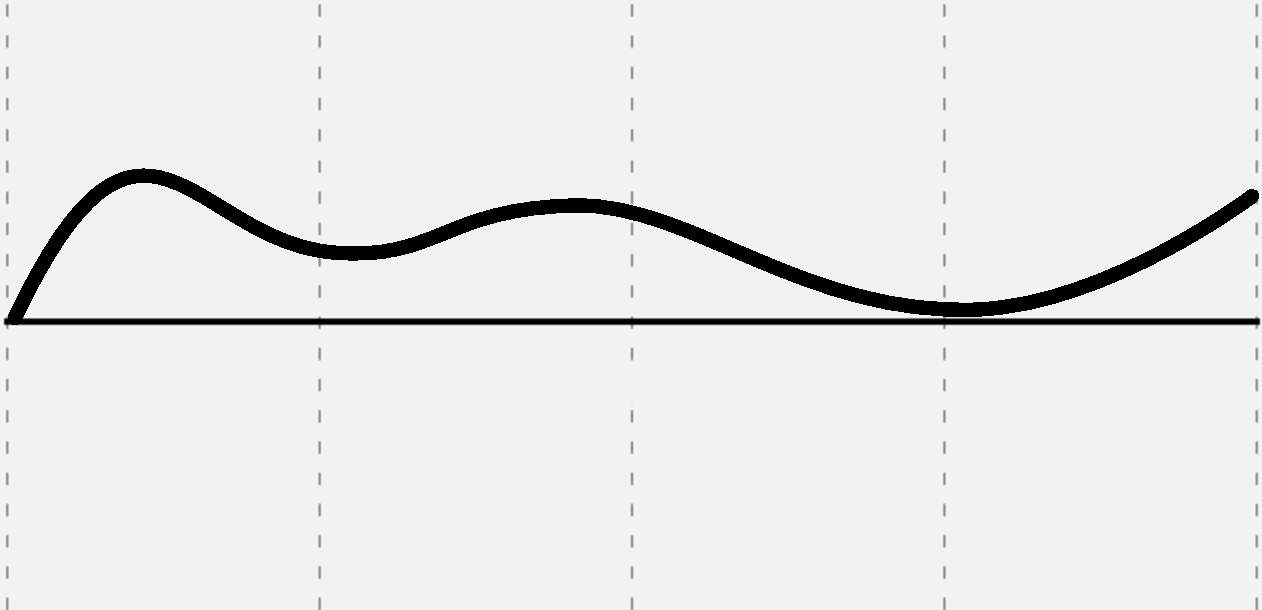
\includegraphics[width=0.25\columnwidth]{img/pattern-indifferent} &
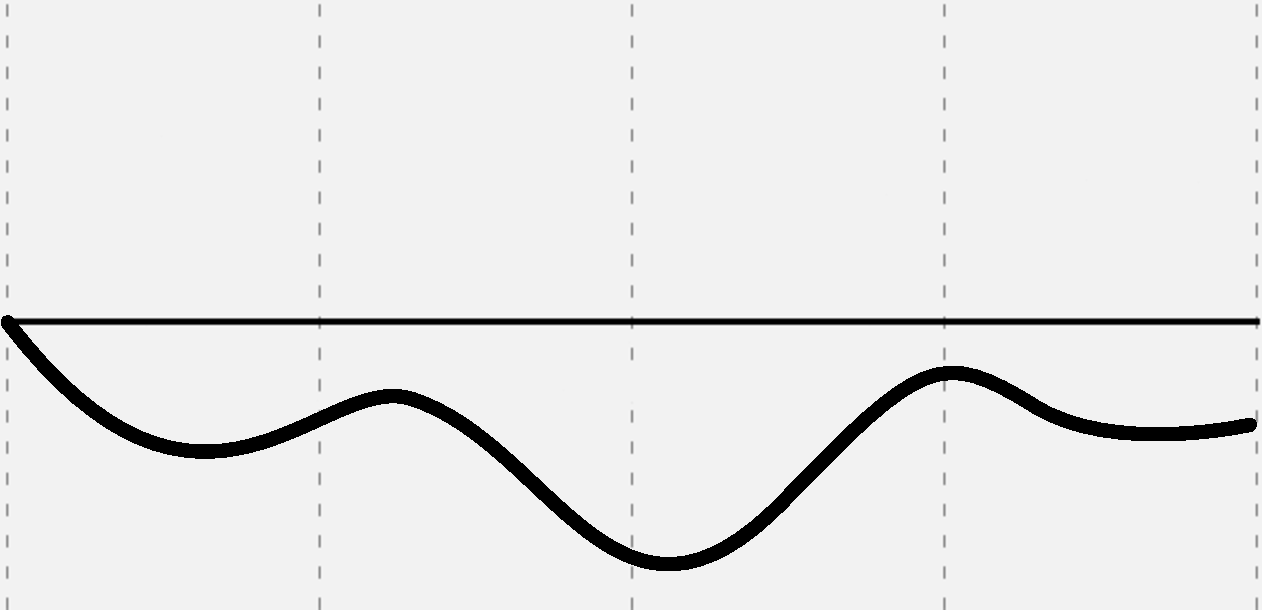
\includegraphics[width=0.25\columnwidth]{img/pattern-discordant} ~ ~&
~ 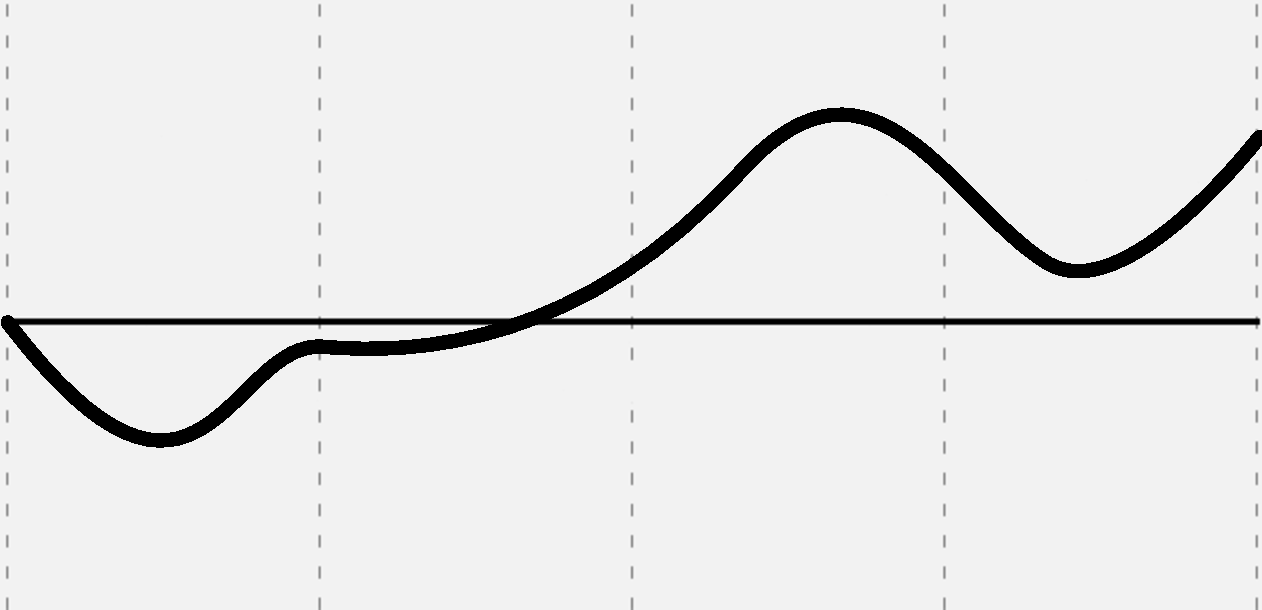
\includegraphics[width=0.25\columnwidth]{img/pattern-textbook-example}\tabularnewline
Indifferent & Discordant & Textbook-example \tabularnewline
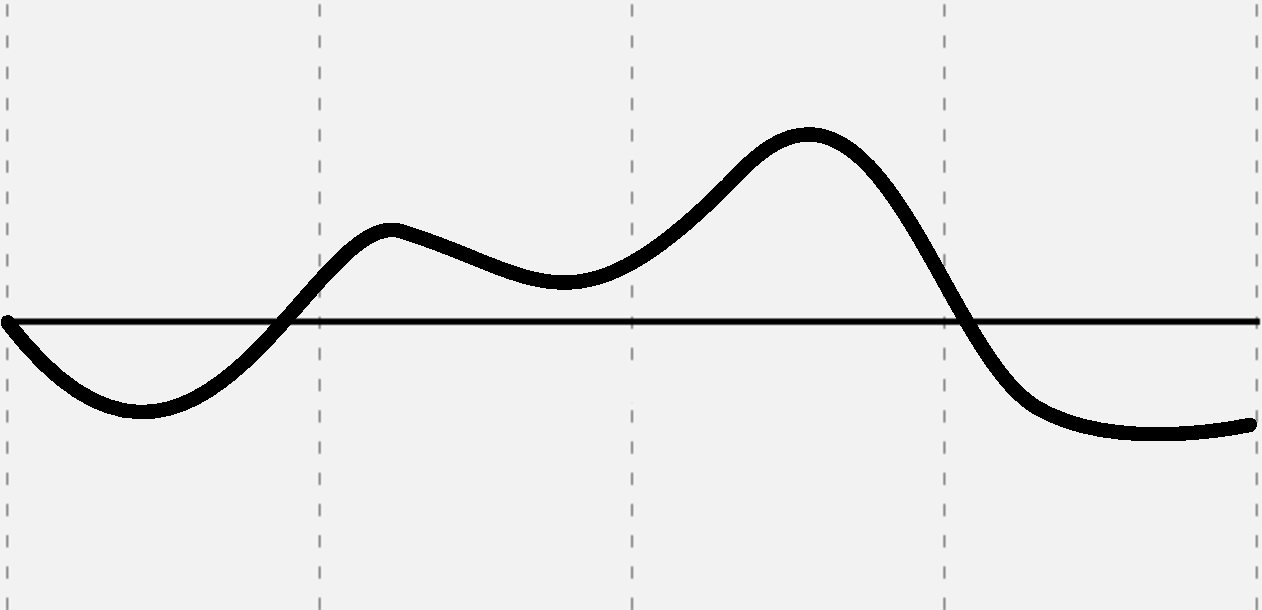
\includegraphics[width=0.25\columnwidth]{img/pattern-back-to-draft} &
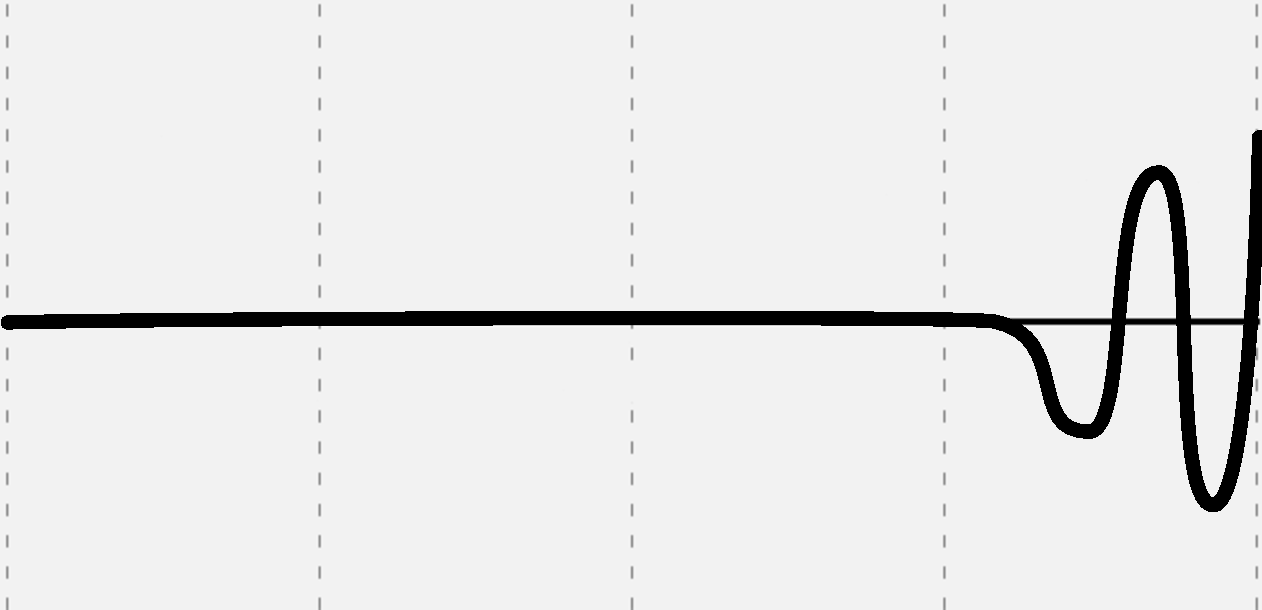
\includegraphics[width=0.25\columnwidth]{img/pattern-procrastination} ~ ~ & 
~ 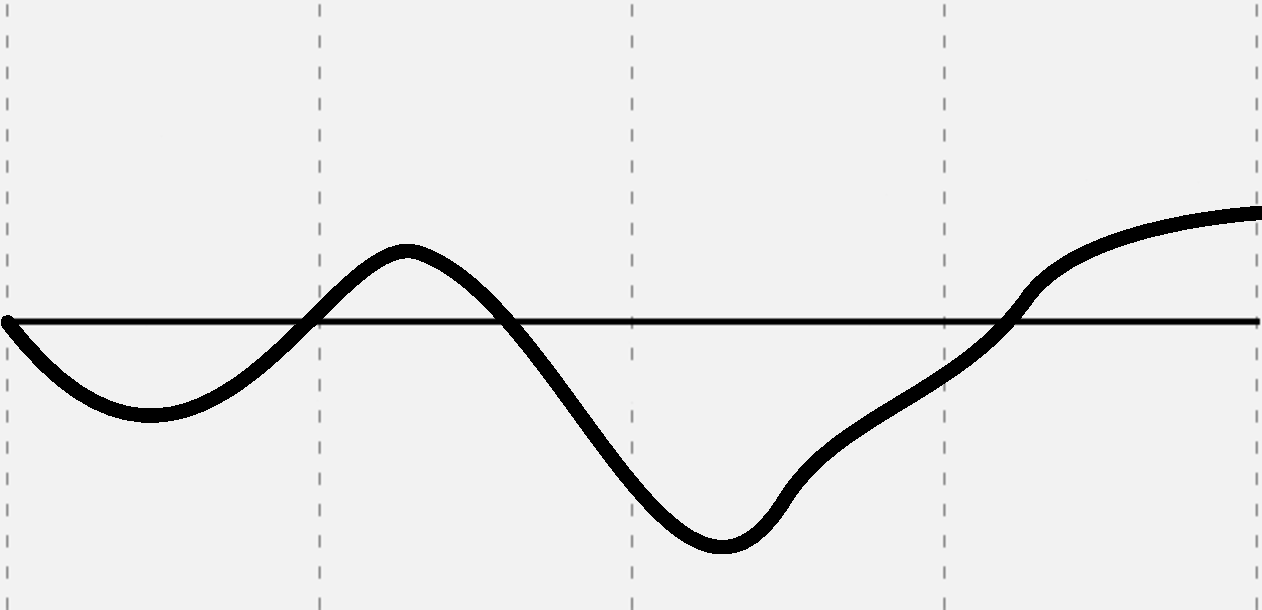
\includegraphics[width=0.25\columnwidth]{img/pattern-happy-ending}
\tabularnewline
Back-to-draft & Procrastination & Happy-ending
\end{tabular}
\end{center}
%
%\vspace{2\columnsep}
%
%
%By this, we help \emph{seeking experts}, \emph{identifying brokers}, \emph{investigating socio-technical congruence}, and \emph{assessing the health of ongoing requirements discussions}.
\end{block}
    
\end{column}
\begin{column}{.45\linewidth}

%{\Large  \color{white} \textsc{\hfill ...Your Potential Benefits}}

%    \begin{block}{Expertise Seeking}
%   \begin{minipage}[c]{.8\linewidth}
%    Analyzing the communication and assignments to tasks related to requirements to help \marker{find experts} for a given topic.
%    \end{minipage}  
%    \hspace{\columnsep}
%    \begin{minipage}[c]{.15\linewidth}
%    
\includegraphics[width=\linewidth]{img/expert-seeking}
%    \end{minipage}
%    \end{block}

%    \vspace{2\columnsep}
%    \begin{block}{Broker Identification}   
%    \begin{minipage}[c]{.4\linewidth}
%    \raggedleft
%    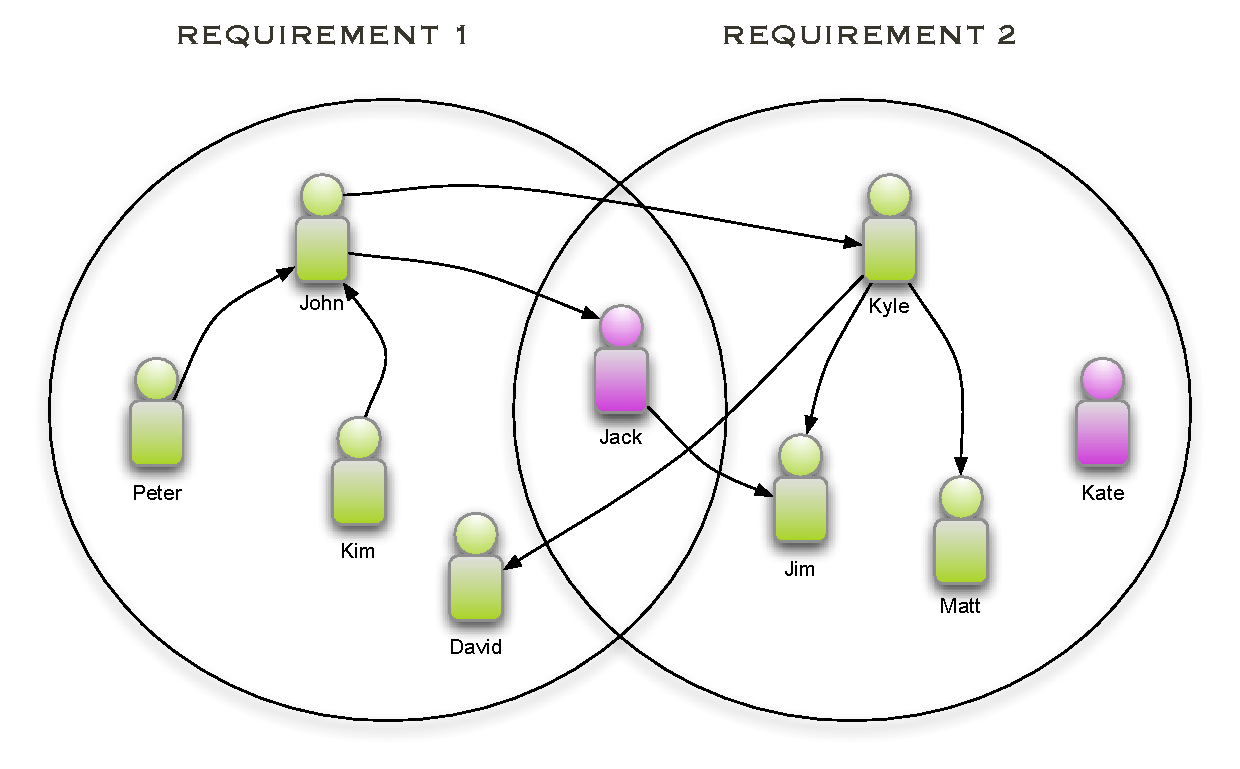
\includegraphics[width=\linewidth]{img/broker}
%    \end{minipage}  
%    \hspace{\columnsep}
%    \begin{minipage}[c]{.5\linewidth}
%  Identifying the brokers of requirements related information to make project managers aware of \marker{critical people} in a project.
%    \end{minipage}    
%    \end{block}
    
%        \vspace{2\columnsep}
    
    %\vspace{\columnsep}
%\vspace{-1cm}

%    \begin{block}{Assessing Socio-technical congruence} 
%    \begin{minipage}[c]{.4\linewidth}
%    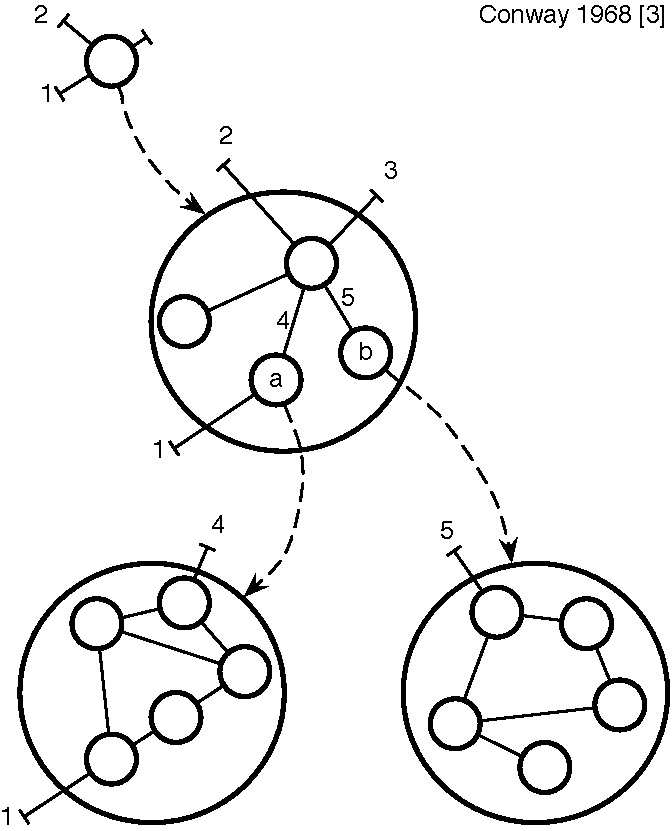
\includegraphics[width=\linewidth]{img/conway}
%    \end{minipage}
%        \hspace{\columnsep}
%   \begin{minipage}[c]{.5\linewidth}
%    Understanding the alignment of the social structure of an organization with the technical dependencies of an organization to allow managers
    
%    \begin{itemize}
%    \item \ldots identifying gaps in coordination.
%    \item \ldots improving collaboration.
%    \end{itemize}
%    \end{minipage}
%   \end{block}
    
%   \vspace{\columnsep}
%  \vspace{2\columnsep}

    \begin{block}{Example}
    Analyzing the content of requirements-related discussion to allow managers \marker{to identify problematic requirements}.
     %   \vspace{2\columnsep}
\begin{center}
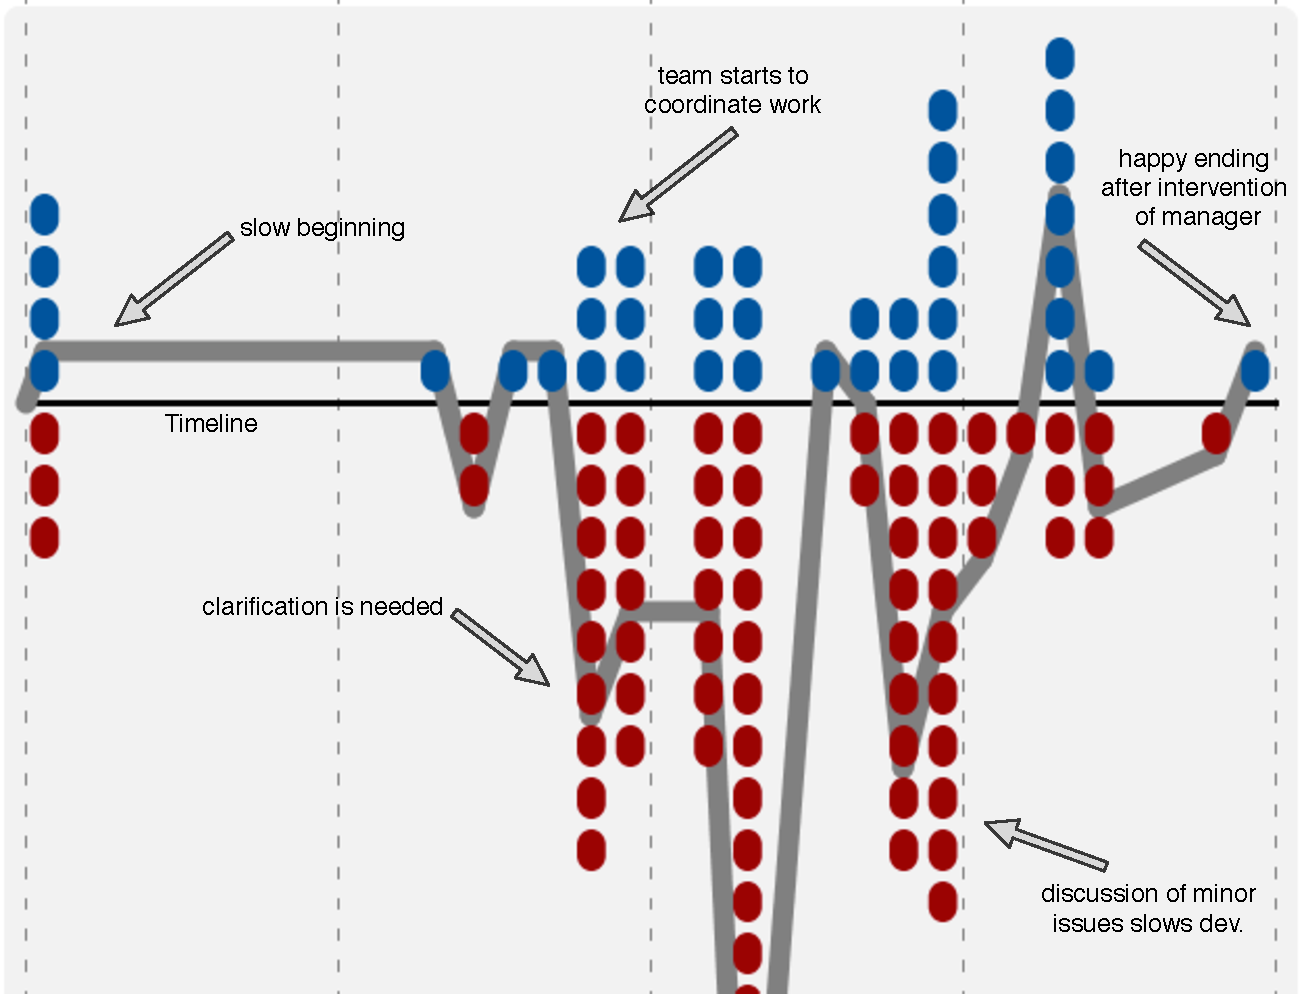
\includegraphics[viewport=0 0 625 475,clip=true,width=0.95\linewidth]{img/bike-shed-example}\\
%\vspace{-0.5cm}
%\hfill \hspace{-1cm} {\tiny *) Thanks to Germán Póo-Caamaño.}
\end{center}


Example trajectory of the discussion related to a user story in a large, globally distributed software project. 
%Preliminary work identified \marker{6 requirements clarification patterns}.
%     \begin{itemize}
%    \item (a) No clarification takes place (Pattern: Indifferent).
%     \item (b) Clarification becomes predominant late in the development of a requirement (Pattern: Back-to-draft).
%     \item (c) Clarification is predominant throughout the development of a requirement (Pattern: Discordant).
%     \item (f) Discussion starts only late in the lifecycle of a requirement (Pattern: Procrastination).
%     \end{itemize}
%\vspace{2\columnsep}
    \end{block}
   

%    \vspace{6\columnsep}
 %   \vspace{0.8cm}
%    \begin{center}
%\colorbox{white}{\parbox{\linewidth}{\centering~ Legend: 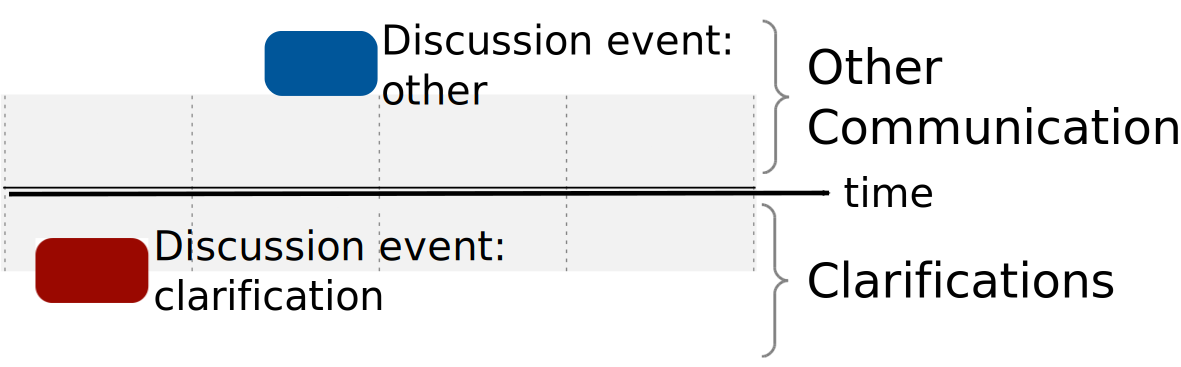
\includegraphics[width=18cm]{img/pattern-legend} ~ }}
%\end{center}
%\vspace{-3cm}

%\begin{exampleblock}{}
%\usebeamercolor*[bg]{block body}
%\usebeamercolor*[fg]{block body}
%Legend: 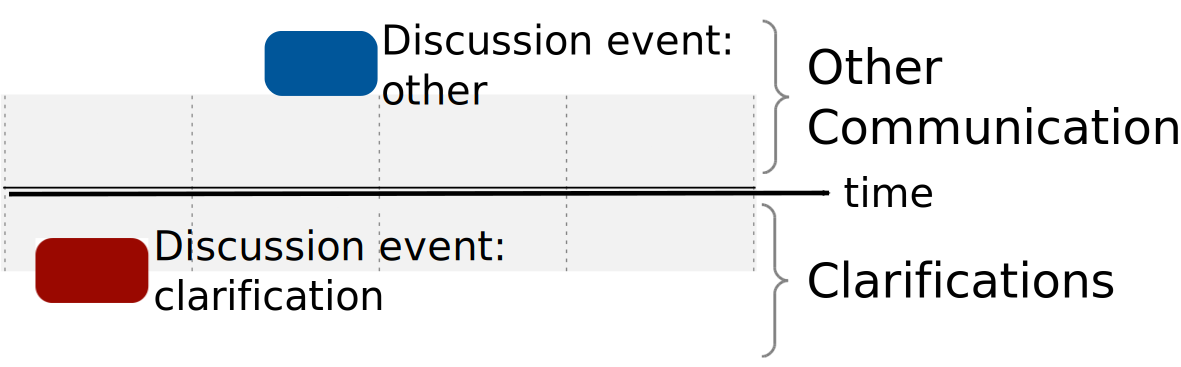
\includegraphics[width=18cm]{img/pattern-legend}
%\end{exampleblock}
    
   %     \vspace{\columnsep}
%\setbeamercolor{postit}{fg=black,bg=white}
%\begin{beamercolorbox}[rounded=true,leftskip=1cm,colsep*=.75ex,wd=\linewidth]{block body}
\begin{block}{Legend}
\begin{center}
\vspace{-0.5cm}
%~ Legend: 
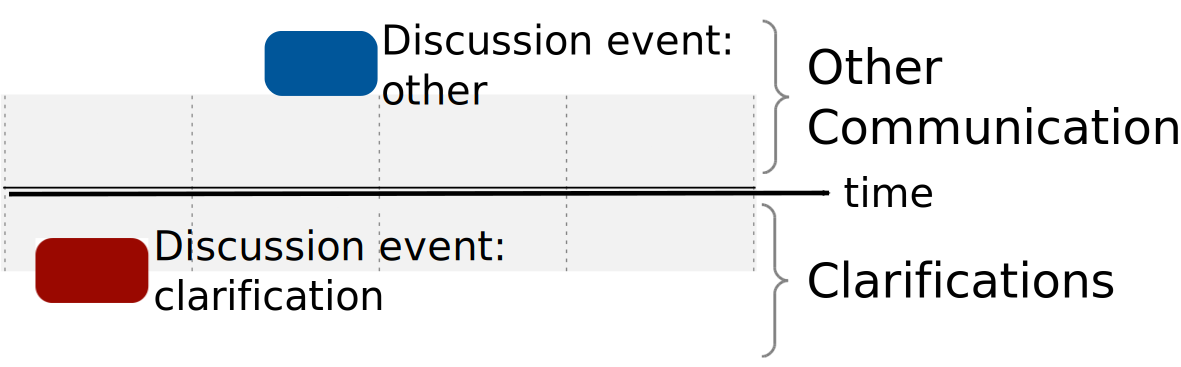
\includegraphics[width=0.9\linewidth]{img/pattern-legend} ~
\end{center}
\vspace{-0.5cm}
\end{block}
%\end{beamercolorbox}

\begin{block}{Voices from Industry  \emph{\footnotesize ~~~~~~IBM RTC, VIATeC}}
\vspace{-0.2cm}
{\small Are these trajectories useful?}
\begin{quote}
\marker{\small“[They...] allow me to find the \\ ~~ones I should focus on.” \\ “I need to know who talks there.”}
\end{quote}
{\small Most valuable before and after feature-complete:}
\begin{quote}
\marker{\small“You shouldn’t clarify things \\~~anymore, then.”}
\end{quote}%
%\vspace{-0.2cm}
\end{block}
\end{column}


\end{columns}

 % \vspace{2\columnsep}
%  \vspace{2\columnsep}


%\hrule
%  \begin{beamercolorbox}[wd=\paperwidth]{upper separation line foot}
%    \rule{0pt}{2pt}
%  \end{beamercolorbox}%
  %
%  \begin{beamercolorbox}[wd=\paperwidth]{footline}
%  \vskip4ex
%  \end{beamercolorbox}%
%
%  \begin{beamercolorbox}[wd=\paperwidth]{lower separation line foot}
  %  \rule{0pt}{2pt}
  %\end{beamercolorbox}
  
 %   \vspace{2\columnsep}


\begin{columns}[b]

% \begin{column}{.45\linewidth}
%   \begin{block}{References}
%    \begin{enumerate}
%    \scriptsize
%    \item Damian, D., Kwan, I., Marczak, S.: Requirements-driven collaboration: Leveraging the invisible relationships between requirements and people. In: Mistrik, I., Grundy, J., Hoek, A., and Whitehead, J. (eds.) Collaborative Software Engineering. 57-76. Springer, Berlin Heidelberg (2010).
%\item Knauss, E., Houmb, S., Schneider, K., Islam, S., J{"u}rjens, J.: Supporting Requirements Engineers in Recognising Security Issues. In: Proceedings of REFSQ’11. Springer, Essen, Germany (2011).
%    \item Conway, M. E.: How Do Committees Invent? In: Datamation magazine. F. D. Thompson Publications, Inc. 1968
%    \end{enumerate}
%    \end{block}
%  \end{column}
  
%  \begin{column}{.199\linewidth}
%  \begin{block}{Acknowledgements}
%   DO WE NEED THIS?
%    \end{block}
%  \end{column}

\begin{column}{0.97\linewidth}
    \begin{block}{Find out how your project can benefit from this}
    \begin{tabular}{v{.45\linewidth}V{0.23\linewidth}V{0.23\linewidth}}
  %  Contact:  
 \vspace{-0.5cm}
    \begin{itemize}
    \item knauss{@}computer.org
 %   \item danielad{@}cs.uvic.ca
    \item http://segal.uvic.ca/
    \end{itemize}
& ~\\ \vspace{-0.5cm}
    
\includegraphics[width=2.5cm]{img/segal-logo_wbg} \\  %\vspace{2\columnsep}
    
\includegraphics[width=2.5cm]{img/uvic-logo_wbg}
& ~\\ \vspace{-0.5cm}
   
\includegraphics[width=1.6cm]{img/segalqrcode}
 \end{tabular}
 
  \vspace{-0.6cm}
    %    \end{block}

%  \end{column}
%  \begin{column}{.199\linewidth}
%    \begin{block}{Affiliation}    
   
  \end{block}

  \end{column}
\end{columns}  

\vfill
\end{frame}

  \end{document}